
% دستوری جهت ظاهر نشدن شماره صفحه و سربرگ، در صورت وجود (فقط در صفحه جاری)
\newpage
\thispagestyle{empty}
\centerline{\includegraphics[scale=0.75]{./Images/general/besmallah.jpg}}

\thispagestyle{empty}
\vspace*{-28mm}
% نحوه درج کردن لوگوی دانشگاه
\centerline{
\includegraphics[scale=0.1]{./Images/general/logo.png}}
\begin{center}
%دستوری برای کم کردن فاصله بین لوگو و خط پایین آن
\vspace{-1mm}
\textbf{دانشکده فنی و مهندسی}
\textbf{گروه مهندسی برق-مخابرات}
%دستوری برای تعیین فاصله بین دو خط
\\[3cm]
\begin{Huge}
\textbf{
بررسی و کاهش کوپلینگ متقابل در آنتن های میکرواستریپ
}
\end{Huge}
\\[1.5cm]
\Large
گزارش پایانی پروژه‌ی کارشناسی
\\[0.25cm]
در رشته‌ی مهندسی برق گرایش مخابرات
\\[3cm]
دانشجو:
\\[0.25cm]
\textbf{
محمد حسن بهشتی    
\\[1cm]
استاد راهنما:
\\[0.25cm]
دکتر حمیدرضا حسنی
\\[1cm]
شهریور ماه ۱۴۰۴
}
\end{center}

\newpage
\thispagestyle{empty}
\centerline{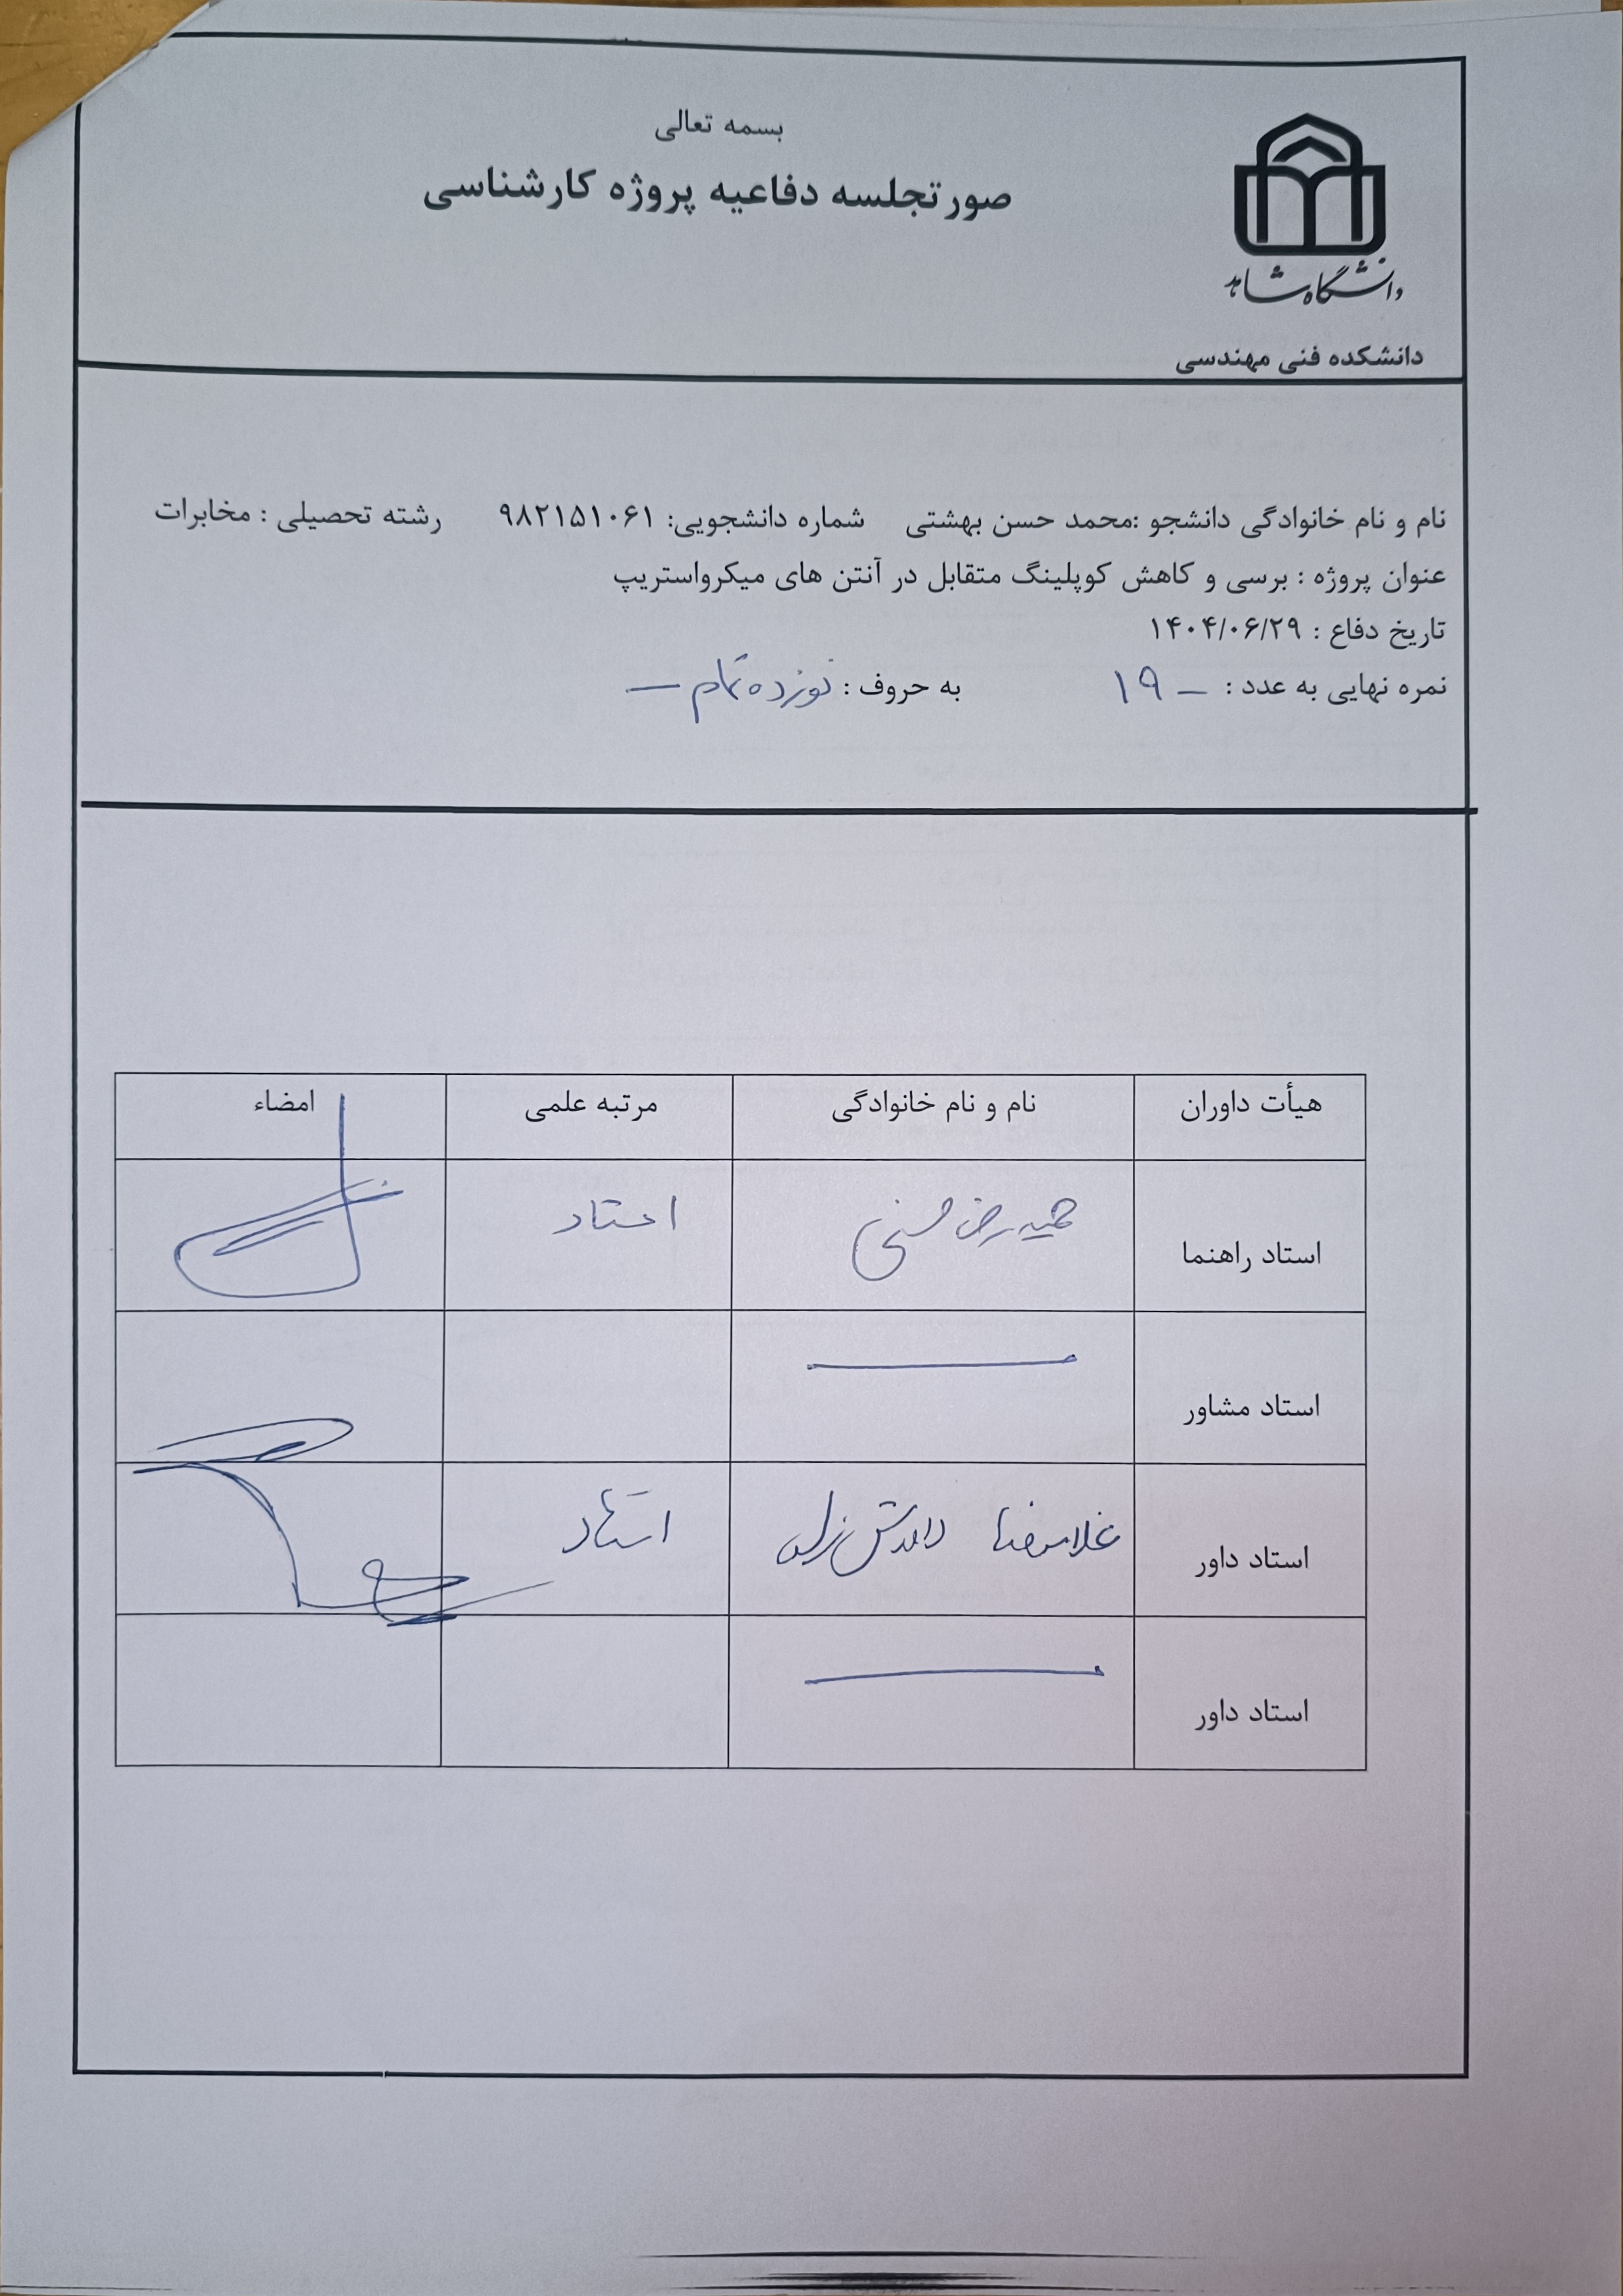
\includegraphics[scale=0.2]{./Images/general/soorat.jpg}}